\documentclass[
    % english, % Klasei padavus parametrą 'english', darbas bus anglų kalba.
    % signatureplaces % prideda parašų vietas tituliniame puslapyje
]{VUMIFPSkursinis}
\usepackage{float}
\usepackage{wrapfig2}
\usepackage{hyperref}
\usepackage{algorithmicx}
\usepackage{algorithm}
\usepackage{algpseudocode}
\usepackage{amsfonts}
\usepackage{amsmath}
\usepackage{bm}
\usepackage{caption}
\usepackage{color}
\usepackage{graphicx}
\usepackage{listings}
\usepackage{subcaption}
\usepackage{biblatex}

\university{Vilniaus universitetas}
\faculty{Matematikos ir informatikos fakultetas}
\department{Programų sistemų studijų programa}
\papertype{Kursinis darbas}
\title{Programų sistemų automatinių testų savaiminio atsistatymo mechanizmų analizė}
\titleineng{Evaluating Self-Healing Mechanisms in Software Test Automation}
\author{Vladimir Deriugin}
\status{4 kurso 2 grupės studentas}
\supervisor{lekt. Dmitrij Nikolajev}
\reviewer{doc. dr. Vardenis Pavardenis}
\date{Vilnius – \the\year}

\bibliography{export}

\begin{document}
\maketitle

\tableofcontents

%% Modifikuotas kursinis.tex failas

\sectionnonum{Įvadas}

Automatizuoti testavimo scenarijai turi būti atnaujinami kaskart, kai programos kūrėjas atlieka pakeitimus programos kode, ypač kai keičiami interneto puslapio elementų atributai, tokie kaip „id“ (identifikatorius), „name“ (vardas) ar „class“ (klasė). Jei šie atributai pasikeičia, testavimo scenarijai gali nebeveikti ir sukelti klaidingų testų nesėkmių. Tokių pakeitimų derinimas yra sudėtingas procesas, reikalaujantis daug laiko ir žmogiškųjų išteklių. Šiame kontekste atsiranda savaiminio atsistatymo (angl. self-healing) mechanizmų idėja. Dirbtinis intelektas identifikuoja neatitikimus esamuose testų scenarijuose ir juos automatiškai pataiso, taip sumažindamas klaidingų nesėkmių tikimybę bei užtikrindamas sklandų testavimo procesą be žmogaus įsikišimo. Šiame darbe analizuojami populiariausi savaiminio atsistatymo įrankiai ir jų efektyvumas praktiniame taikyme

\textbf{Tyrimo objektas} $-$ Savaiminio atsistatymo įrankiai, kurie siūlo skirtingus sprendimus, kaip testai gali savarankiškai aptikti ir ištaisyti klaidas, atsirandančias dėl sąsajos, DOM struktūros, API ar kitų elementų pokyčių.

\textbf{Darbo tikslas} $-$  išsiaiškinti, kaip savaiminio atsistatymo mechanizmas padeda greičiau ir patikimiau automatizuoti programų testavimą.

\textbf{Darbo uždaviniai :} 
 
\begin{enumerate} 
    \item Ištirti klaidų aptikimo ir taisymo būdus testuose, atsirandančius dėl pokyčių sąsajoje, DOM struktūroje, API ir kituose testuojamos sistemos elementuose.
    \item Atlikti savaiminio atsistatymo mechanizmų palyginimą pasirinktuose įrankiuose, įvertinant jų tikslumą, atstatymo greitį ir klaidingų teigiamų rezultatų skaičių.
    \item Įvertinti šių mechanizmų poveikį testų scenarijų stabilumui ir palaikymui, taip pat laikui ir ištekliams, skiriamiems testų palaikymui, sumažinimui.
\end{enumerate}

\textbf{Tyrimo metodai}

Siekiant tikslų ir išspręsti uždavinius, šioje darbe bus naudojami šie tyrimo metodai:

\begin{enumerate}
    \item \textbf{Palyginamoji analizė}: Analizuoti savaiminio atstatimo įrankių platformų funkcionalias galimybes ir savaiminio atsistatymo mechanizmus, įvertinant jų stipriąsias ir silpnąsias puses.
    \item \textbf{Eksperimentiniai tyrimai}: Vykdyti kontroliuojamus eksperimentus naudojant realius testavimo scenarijus ir taikymus, atlikti pokyčius testuojamame taikyme ir stebėti platformų elgesį atkuriant testus.
    \item \textbf{Veikimo ir metrikų analizė}: Rinkti ir analizuoti kiekybinius duomenis, susijusius su savaiminio atsistatymo mechanizmų veikimu, tokius kaip testų atkūrimo laikas, taisymų tikslumas ir klaidingų teigiamų rezultatų skaičius.
\end{enumerate}

\textbf{Darbo struktūra}
\begin{enumerate}
    \item \textbf{Įvadas}, kuris aptaria temos aktualumą, formuluoja tyrimo tikslus ir uždavinius, taip pat aprašo tyrimo objektą, metodus ir darbo struktūrą.
    \item \textbf{Automatinių testų kontekstas} - nagrinėja automatizuoto testavimo raidą, regresinio testavimo svarbą ir savaiminio atsistatymo mechanizmų atsiradimą.
    \item \textbf{Savaiminis atsistatymas ir teoriniai pagrindai} - aprašomi savaiminio atsistatymo veikimo principai, jų tipai bei teoriniai pagrindai.
    \item \textbf{Esamų sprendimų apžvalga ir palyginimas} - analizuojami populiariausi savaiminio atsistatymo įrankiai, jų veikimo metodai, pritaikymo galimybės bei iššūkiai.
    Atliekama išsami skirtingų įrankių palyginamoji analizė, apimanti klaidų aptikimo ir taisymo tikslumą, atstatymo greitį ir poveikį testavimo procesui.
    \item \textbf{Eksperimentas} - pateikiama eksperimento metodika, gauti rezultatai ir jų interpretacija.
    \item \textbf{Rezultatai ir išvados} apibendrina tyrimo metu surinktus duomenis, išskiria pagrindines įžvalgas bei pateikia rekomendacijas testavimo specialistams, taip pat nurodo galimas tolesnių tyrimų kryptis.
\end{enumerate}

Šis kursinis darbas suteikia gilų supratimą apie savaiminio atsistatymo mechanizmų praktinį pritaikymą bei jų efektyvumą testavimo automatizavimo kontekste.

\section{Literatūros atrankos metodika ir analizė}

Atliekant literatūros analizę šiam darbui, buvo nuspręsta taikyti struktūrizuotą ir sistemingą metodiką, siekiant efektyviai surinkti ir apdoroti aktualius šaltinius. Ši strategija leido sutelkti dėmesį į mokslinius straipsnius ir tyrimus, kurie tiesiogiai susiję su programinės įrangos automatizuotu testavimu ir savaiminio atsistatymo mechanizmais.

\subsection{Literatūros paieškos strategija}

Savaiminio atsistatymo literatūros paieškai buvo nuspręsta naudoti aiškiai apibrėžtus kriterijus, siekiant efektyviau struktūrizuoti paieškos procesą ir išvengti nereikalingos informacijos. Šis metodas leido susitelkti tik į tuos šaltinius, kurie tiesiogiai atitinka darbo temą.

Pradinėje literatūros atrankos fazėje buvo aiškiai apibrėžtos tyrimo ribos ir tikslai:

\begin{itemize}
    \item \textbf{Tematinė sritis:} programinės įrangos testavimo automatizacija ir savaiminio atsistatymo mechanizmai.
    \item \textbf{Laiko apribojimas:} paskutinių 12 metų moksliniai leidiniai, užtikrinant šaltinių aktualumą.
    \item \textbf{Publikacijos tipas:} recenzuoti moksliniai straipsniai, informacines technologijos straipsniai, techninės ataskaitos bei konferencijų medžiaga.
\end{itemize}

Paieška buvo vykdoma šiose duomenų bazėse:

\begin{enumerate}
    \item \textbf{IEEE Xplore –} dėl stiprios orientacijos į inžinerinius ir technologinius tyrimus.
    \item \textbf{ACM Digital Library –} kaip viena iš pagrindinių kompiuterių mokslų tyrimų platformų.
    \item \textbf{SpringerLink ir ScienceDirect – } plataus spektro mokslinės literatūros šaltiniai.
    \item \textbf{Google Scholar –} papildomas įrankis, užtikrinantis plačią prieigą prie įvairių publikacijų.
\end{enumerate}

Naudoti raktažodžiai buvo parinkti taip, kad padėtų eliminuoti nereikalingus rezultatus ir užtikrintų paieškos tikslumą:

\begin{itemize}
    \item \textit{“software testing automation”} AND \textit{"self-healing mechanisms"} – siekiant sutelkti dėmesį į automatizuotą testavimą.
    \item \textit{“test maintenance efficiency”} AND \textit{“automated tools”} – orientuota į testavimo procesų optimizavimą.
    \item \textit{“machine learning in software testing”} – skirtas identifikuoti mašininio mokymosi taikymus automatizacijoje.
    \item \textit{“adaptive recovery algorithms”} – siekiant atrasti algoritmus, susijusius su savaiminiu atsistatymu.
\end{itemize}

Šis raktažodžių pasirinkimas buvo būtinas, nes vien tik “self-healing” sąvoka dažnai nurodo į medicinos ar medžiagų mokslo publikacijas, kurios nėra susijusios su šio darbo tema. Papildomi raktažodžiai užtikrino, kad paieškos rezultatai būtų tiksliniai ir tiesiogiai susiję su tyrimo klausimais.

\subsection{Atrankos kriterijai}

Siekiant išlaikyti darbo mokslinį pagrįstumą, literatūros atranka buvo vykdoma laikantis aiškių ir tikslių kriterijų:

\begin{enumerate}
    \item \textbf{Metodologinis pagrįstumas –}  prioritetas teiktas darbams, pateikiantiems aiškius eksperimentinius duomenis, algoritmų aprašus ar teorinius modelius.
    \item \textbf{Publikacijos kokybė –  } buvo vertinamos tik recenzuotos publikacijos.
    \item \textbf{Cituojamumo rodikliai –} straipsniai, turintys aukštą cituojamumo indeksą, buvo laikomi patikimesniais.
\end{enumerate}

\subsection{Analizės metodika}

Surinkti šaltiniai buvo sistemingai analizuojami, laikantis tokios procedūros:

\begin{enumerate}
    \item \textbf{Santraukų analizė}  išsamiau įvertinti tik tie darbai, kurių santraukos atitiko tyrimo klausimus.
    \item \textbf{Turinio žymėjimas –  } naudotos anotacijų kūrimo programos "Mendeley", siekiant išryškinti pagrindines sąvokas, idėjas ir algoritmus.
    \item \textbf{Kokybinė analizė –} išskirtos pagrindinės temos: testų stabilumo gerinimas, automatizavimo įrankių veikimo palyginimas ir mašininio mokymosi taikymas savaiminiam atsistatymui.
\end{enumerate}

\section{Automatinių testų kontekstas}

Automatizuotas programinės įrangos testavimas yra vienas pagrindinių kokybės užtikrinimo proceso elementų, leidžiantis efektyviai nustatyti ir pašalinti klaidas programiniuose sprendimuose. Pastaraisiais metais šis procesas tapo ypač aktualus dėl sparčiai augančio programinės įrangos sudėtingumo, trumpėjančių vystymo ciklų bei vis didėjančių vartotojų reikalavimų dėl kokybės \cite{myers2011} Automatizuotas testavimas leidžia žymiai sumažinti rankinio darbo kiekį, padidinti testavimo apimtį bei pasiekti nuoseklius rezultatus \cite{meszaros2007}

Nepaisant reikšmingų pranašumų, automatizuoto testavimo įgyvendinimas ir palaikymas kelia daug iššūkių. Vienas didžiausių sunkumų yra susijęs su automatizuotų testų patikimumu. Testavimo aplinkoje dažnai įvyksta pokyčių, tokių kaip vartotojo sąsajos modifikacijos, infrastruktūros atnaujinimai ar netikėti klaidų scenarijai, kurie gali sukelti testų gedimus. Šie gedimai neretai yra klaidingi, nes jie nurodo ne į programinės įrangos problemas, o į pasenusius ar netinkamai sukonfigūruotus testus. Dėl to testų palaikymas tampa daug laiko reikalaujančiu ir brangiu procesu, kuris gali sumažinti automatizavimo teikiamą naudą.

\subsection{Automatizuoto testavimo raida ir svarba}

Automatizuoto testavimo istorija prasidėjo dar praėjusio amžiaus aštuntajame dešimtmetyje, kai buvo sukurti pirmieji įrankiai, leidžiantys automatizuoti paprasčiausius testavimo procesus \cite{fowler2018}. Iš pradžių šie įrankiai buvo naudojami tekstinėms vartotojo sąsajoms testuoti, tačiau augant kompiuterinės technikos pajėgumams ir programinės įrangos sudėtingumui, atsirado pažangesni metodai ir įrankiai, skirti įvairių sistemų ir platformų testavimui \cite{koranne2010}

Dešimtajame dešimtmetyje automatizuotas testavimas įgijo didesnį populiarumą, kai programinės įrangos vystymo procesai pradėjo remtis iteraciniais metodais, tokiais kaip Agile ir Scrum \cite{cohn2009}. Tai paskatino testavimo įrankių evoliuciją ir didesnę integraciją su vystymo aplinkomis. Pasirodė įrankiai, gebantys automatizuoti ne tik tekstines vartotojo sąsajas (angl. UI), bet ir aplikacijų programavimo sąsajas (angl. API) bei svetainių aplikacijas.

2000-aisiais metais testavimo pramonėje įvyko reikšmingas šuolis: pradėjo formuotis atvirojo kodo įrankių ekosistemos, tokios kaip Selenium, kurios leido sumažinti testavimo kaštus ir išplėsti automatizavimo galimybes \cite{Selenium2023}. Šie įrankiai tapo pagrindine daugelio organizacijų testavimo proceso dalimi.

Pastaraisiais metais automatizuotas testavimas transformavosi į sudėtingą procesą, apimantį dirbtinio intelekto ir mašininio mokymosi technologijas. Šios technologijos leidžia dar labiau sumažinti rankinio darbo poreikį, prognozuoti galimus klaidų scenarijus bei automatiškai prisitaikyti prie dinamiškų testavimo aplinkų \cite{Testim} Testavimo įrankiai tapo proaktyviais, gebančiais analizuoti sistemos pokyčius ir pasiūlyti optimizacijas.

Modernus automatizuotas testavimas remiasi trimis pagrindiniais tipais, kurie išdėstomi pagal API ir UI testavimo piramidę:
\begin{enumerate}
    \item \textbf{Vieneto testavimas (angl. Unit Testing):} tai pagrindinis piramidės lygmuo, skirtas atskirų programos komponentų veikimo tikrinimui. Jis užtikrina, kad kiekviena programos dalis veiktų teisingai nepriklausomai nuo kitų \cite{meszaros2007}.
    \item \textbf{Integracinis testavimas (angl. Integration Testing):} šis tarpinis piramidės lygmuo tikrina, kaip skirtingi komponentai veikia kartu. Tai ypač svarbu, kai komponentai turi dalintis duomenimis ar bendrauti tarpusavyje \cite{fowler2018}.
    \item \textbf{Vartotojo sąsajos testavimas (angl. UI Testing):} aukščiausias piramidės lygmuo, skirtas visos sistemos tikrinimui realiomis naudojimo sąlygomis, ypač per vartotojo sąsają. Šis lygmuo dažnai reikalauja daugiausiai resursų ir laiko, tačiau yra būtinas, kad būtų užtikrintas teisingas galutinio produkto veikimas \cite{meszaros2007}.
\end{enumerate}

Šie testavimo tipai sudaro vadinamąją API ir UI testavimo piramidę:

\begin{figure}[H]
    \centering
    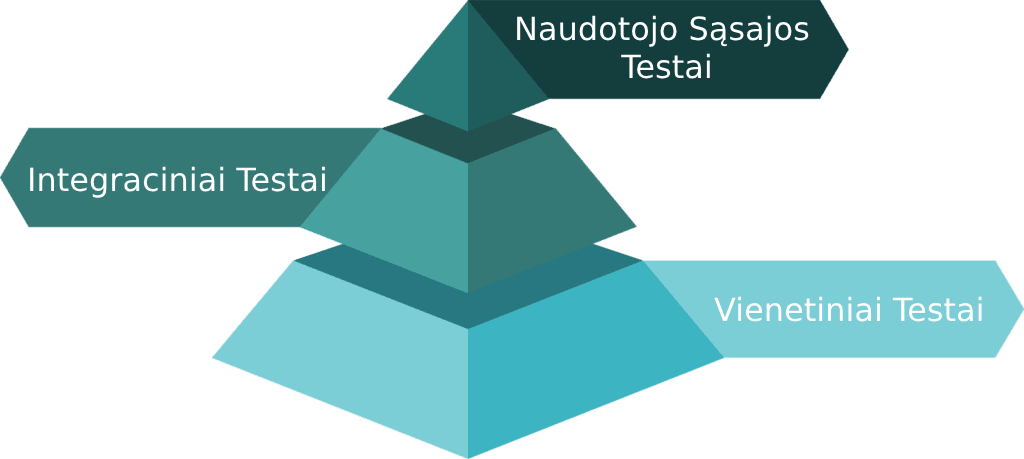
\includegraphics[scale=0.25]{img/Piramide.png}
    \caption{Testavimo piramidę}
    \label{img:piramide}
\end{figure}

\subsection{Regresinio testavimo svarba ir iššūkiai}

Regresinis testavimas yra vienas svarbiausių automatizuoto testavimo tipų, užtikrinantis, kad naujai atlikti programinės įrangos pakeitimai nesugadintų esamų funkcionalumų. Šis procesas ypač reikšmingas judrių vystymo ciklų metu, kai programinės įrangos iteracijos vyksta dažnai ir greitai \cite{kaner2002}. Regresinis testavimas leidžia aptikti klaidas, kurios gali atsirasti dėl netikėtų sąveikų tarp naujų ir esamų kodo dalių \cite{black2009}.

Šio testavimo tikslas yra patikrinti, ar atlikti pakeitimai nesukėlė šalutinių poveikių visai sistemai. Dažniausiai regresinis testavimas apima iš anksto sukurtus automatizuotus testų rinkinius, kurie apima pagrindines sistemos funkcijas \cite{fewster1999}. Tačiau regresinio testavimo palaikymas kelia daug problemų, nes dažni sistemos ar vartotojo sąsajos pakeitimai lemia, kad testai tampa neveiksmingi ir juos reikia atnaujinti \cite{whittaker2000}.

Testų neveiksmingumas dažnai atsiranda dėl "klaidingų teigiamų" rezultatų, kai testai praneša apie problemas, nors realiai jų nėra. Tai prailgina klaidų analizės laiką ir gali sumažinti pasitikėjimą testavimo procesais \cite{fewster1999}. Be to, rankinis testų atnaujinimas yra sudėtingas ir daug laiko reikalaujantis procesas, kuris užkrauna didelę naštą testavimo komandoms \cite{black2009}. Todėl vis svarbesnis tampa automatizuotas testų atnaujinimas ir savarankiškos sistemos, kurios gali prisitaikyti prie pokyčių, užtikrinant nuolatinį testavimo proceso efektyvumą \cite{kaner2002}.

Daugelis organizacijų susiduria su situacija, kai regresinio testavimo palaikymas suvartoja didžiąją dalį testavimo komandos resursų. Rankinis testų atnaujinimas ne tik atima daug laiko, bet ir padidina klaidų riziką. Šiuo atveju svarbų vaidmenį atlieka modernūs įrankiai ir metodai, galintys automatizuoti šį procesą bei sumažinti darbo krūvį \cite{whittaker2000}.

\subsection{Savaiminio atsistatymo mechanizmų atsiradimas}

Siekiant spręsti šiuos iššūkius, pastaruoju metu atsirado savaiminio atsistatymo (angl. self-healing) mechanizmai, kurie yra skirti testų patikimumui ir palaikymo efektyvumui didinti. Šie mechanizmai leidžia automatizuoti testų prisitaikymą prie aplinkos pokyčių, identifikuoti ir taisyti klaidingus gedimus bei minimizuoti žmogaus įsikišimo poreikį \cite{eck2020}.

Automatizuoto testavimo specialistai susiduria su poreikiu nuolat stebėti ir analizuoti testų veikimą, identifikuoti pagrindines gedimų priežastis bei užtikrinti, kad visi testai veiktų sklandžiai. Dėl šios priežasties savaiminio atsistatymo technologijos tampa svarbia priemone, padedančia sumažinti testavimo komandos darbo krūvį ir užtikrinti, kad programinė įranga būtų testuojama greitai ir patikimai \cite{zimmermann2019}.

Aptarsime šių technologijų teorinius pagrindus, jų esamus sprendimus bei veiksmingumą. Tikslas yra parodyti, kaip savaiminio atsistatymo mechanizmai gali pagerinti automatizuoto testavimo procesus ir prisidėti prie efektyvesnio programinės įrangos kokybės užtikrinimo \cite{harman2012}.

\section{Savaiminio atsistatymo teoriniai pagrindai}

Savaiminis atsistatymas (angl. self-healing) yra metodika, kurios tikslas yra užtikrinti, kad automatizuotas testavimas veiktų patikimai ir efektyviai, net kai testavimo aplinkoje įvyksta pokyčiai. Šis mechanizmas suteikia sistemoms gebėjimą automatiškai identifikuoti ir ištaisyti problemas be žmogaus įsikišimo, taip sumažinant rankinio darbo poreikį ir užtikrinant sklandų testavimo procesą \cite{lemos2020} \cite{camara2019}.

\subsection{Kaip veikia savaiminis atsistatymas}

Savaiminis atsistatymas yra viena iš pažangiausių metodikų automatizuotame testavime, leidžianti sistemoms prisitaikyti prie pokyčių be žmogaus įsikišimo. Jos veikimas grindžiamas gebėjimu analizuoti, atpažinti ir koreguoti klaidas, atsirandančias dėl programinės įrangos ar aplinkos pokyčių \cite{lemos2020}. Toliau aprašomi etapai, kurie sudaro šios metodikos pagrindą:

\subsubsection{Elemento identifikavimas (angl. Identifying the Element):} Pirmasis ir svarbiausias žingsnis savaiminio atsistatymo procese yra elementų identifikavimas. Šis procesas yra kur kas sudėtingesnis nei tradicinio automatizuoto testavimo, kuris dažnai remiasi vienu atributu. Savaiminio atsistatymo įrankiai kaupia įvairius atributus, tokius kaip identifikatorius (ID), pavadinimas, CSS selektorius, XPath ir tekstas, taip pat elementų santykinę padėtį kitų elementų atžvilgiu \cite{camara2019}.

Šis daugialypis požiūris suteikia įrankiui gilesnį kiekvieno elemento supratimą, užtikrinant, kad testai galėtų nuosekliai identifikuoti elementus, net jei tam tikri atributai buvo pakeisti. Tokiu būdu žymiai padidėja testavimo prisitaikymas prie programinės įrangos pokyčių.
    
\subsubsection{Organizuotas testų vykdymas (angl. Organized Test Execution):} Savaiminis atsistatymas vykdomas pagal iš anksto suplanuotą testų scenarijų, sąveikaujant su konkrečiomis tinklalapio dalimis ir prisitaikant prie mažų svetainių elementų pokyčių. Pavyzdžiui, jei testas apima mygtuko paspaudimą, savaiminio atsistatymo įrankis pirmiausia ieško mygtuko naudodamas pagrindinį identifikatorių, pvz., elemento identifikatorių. Šis metodas leidžia tiksliai vykdyti testus pagal pradinį scenarijų, užtikrinant programinės įrangos funkcionalumo vertinimą nurodytose situacijose \cite{garlan2004}.
    
\subsubsection{Problemos identifikavimas ir analizė (angl. Issue Identification and Analysis):} Jei testas negali rasti elemento naudodamas pagrindinį identifikatorių dėl programinės įrangos pakeitimų, įrankis nepraneša apie gedimą iš karto. Vietoj to, jis inicijuoja problemos diagnostikos procesą. Šio etapo metu įrankis naudoja atsarginius metodus, siekdamas surasti trūkstamą elementą, naudodamas antrinius identifikatorius ar atributus, užregistruotus pirminio testo kūrimo metu \cite{harman2012}. Taip pat gali būti pasitelkta elemento padėtis, lyginant su stabiliais puslapio elementais, kas leidžia užtikrinti testavimo tęstinumą.

\subsubsection{Savaiminis atsistatymas (Self Healing):} Pagrindinė savaiminio atsistatymo esmė slypi jo gebėjime mokytis ir prisitaikyti. Jei įrankis sėkmingai randa elementą naudodamas alternatyvų metodą, jis atnaujina pradinį testų scenarijų, įtraukdama naują vertę. Tai leidžia atlikti efektyvesnius ateities testus ir sumažina panašių problemų tikimybę. Šis tęstinio mokymosi procesas palaiko testų veiksmingumą ir užtikrina jų prisitaikymą prie pokyčių laikui bėgant \cite{garlan2004}.

\subsection{Savaiminio atsistatymo tipai}

Savaiminis atsistatymas yra sudėtingų programinės įrangos testavimo procesų dalis, kuri orientuota į testavimo stabilumo užtikrinimą dinamiškai besikeičiančiose aplinkose. Kuriantis šiai technologijai, atsirado poreikis klasifikuoti metodus pagal jų veikimo principus ir sudėtingumą. Toliau pateikiama pagrindinių savaiminio atsistatymo metodų klasifikacija.

\subsubsection{Heuristiniai mechanizmai:} Šie mechanizmai remiasi taisyklėmis ir algoritmais, kurie iš anksto apibrėžia, kaip sistema turėtų reaguoti į tam tikrus pokyčius. Heuristinis metodas yra paprastas ir efektyvus, tačiau jo taikymas yra ribotas, kai testavimo aplinka yra labai dinamiška ar kompleksiška \cite{lewis2010}. Šis metodas buvo vienas pirmųjų savaiminio atsistatymo sprendimų, pasirodžiusių tuo metu, kai automatizuotas testavimas tik pradėjo vystytis.
    
\subsubsection{Dirbtinio intelekto mechanizmai:} Šie mechanizmai naudoja mašininio mokymosi algoritmus, kurie geba analizuoti didelius duomenų kiekius, identifikuoti modelius ir prisitaikyti prie pokyčių. Dirbtinio intelekto (toliau DI) tipo savaiminis atsistatymas yra daug pažangesnis, nes jis leidžia sistemai mokytis iš patirties ir nuolat tobulėti. Tai taip pat leidžia greitai reaguoti į sudėtingesnius ir nenumatytus pokyčius.

Šiuolaikinėje praktikoje DI tipo savaiminis atsistatymas yra vis dažniau naudojamas, nes jis užtikrina didesnį testavimo efektyvumą ir sumažina klaidingų teigiamų rezultatų skaičių. Šis kursinis darbas koncentruosis būtent į DI tipo savaiminį atsistatymą, jo galimybes ir poveikį automatizuotam testavimui.

Heuristiniai metodai dažniausiai naudojami paprastesniuose scenarijuose, o dirbtinio intelekto mechanizmai yra skirti sudėtingoms ir dinamiškoms sistemoms, kur reikalingas aukštas prisitaikymo lygis \cite{goodfellow2016}.

\section{Esamų sprendimų apžvalga ir palyginimas}

Dabartinėje rinkoje jau veikia keletas savaiminio atsistatymo sprendimų. Tokie įrankiai kaip Healenium, Applitools, Mabl ar Testim siūlo skirtingus metodus ir technologijas, padedančias automatizuoti testų atnaujinimą, pagerinti stabilumą ir sumažinti testų palaikymo sąnaudas.

\subsection{Healenium} 

Healenium yra atvirojo kodo įrankis, integruojantis savaiminio atsistatymo funkcionalumą į populiarų testavimo karkasą Selenium. Pasak \cite{Khankhoje2023}, Healenium naudoja DI ir MM algoritmus, kad automatiškai koreguotų testų scenarijus, kai keičiasi svetainės elementai. Šio įrankio privalumas yra jo integracija su plačiai naudojamu Selenium, leidžianti naudotojams lengvai pritaikyti savaiminio atsistatymo funkcijas esamuose testų rinkiniuose. Tačiau Healenium gali susidurti su iššūkiais, kai pokyčiai yra labai dideli arba netipiniai, o tai gali riboti jo efektyvumą sudėtingose aplinkose. \cite{Healenium}

\subsubsection{Klaidos aptikimo ir taisymo būdai}

Healenium integruojasi su Selenium, suteikdamas galimybę automatiškai aptikti ir taisyti pokyčius vartotojo sąsajoje (angl. UI), DOM struktūroje ir API. Naudodamas dirbtinį intelektą ir mašininį mokymąsi (toliau MM), Healenium gali automatiškai atnaujinti testų lokatorius, kai jie pasikeičia. Šis mechanizmas leidžia testams prisitaikyti prie dinamiškų sąsajų pokyčių be rankinio įsikišimo.

\subsubsection{Savaiminio atsistatymo mechanizmų tikslumas ir greitis}

Healenium pasižymi aukštu tikslumu taisant lokatorius, nes jis naudoja pažangius DI algoritmus, kurie analizuoja elementų atributus ir kontekstą. Atstatymo greitis yra greitas, nes testai gali būti atkuriami beveik realiu laiku, leidžiantys sumažinti testavimo ciklų trukmę. Tačiau kai kuriuose sudėtinguose scenarijuose gali pasitaikyti klaidingų teigiamų rezultatų, kai lokatoriai netinkamai atnaujinami dėl neaiškių elementų pokyčių.

\subsubsection{Poveikis testų scenarijų stabilumui ir palaikymui}

Integruojant Healenium, testų scenarijų stabilumas ženkliai pagerėja, nes automatiniai atnaujinimai sumažina nesėkmių skaičių dėl vartotojo sąsajos (angl. UI) pokyčių. Tai taip pat sumažina laiką ir išteklius, reikalingus testų priežiūrai, leisdami testavimo komandoms sutelkti dėmesį į kitus svarbius uždavinius. Healenium prisideda prie efektyvesnio testavimo proceso, mažindamas rankinio atnaujinimo poreikį.

\subsection{Applitools}

Applitools specializuojasi vizualiniame testavime, naudodama kompiuterinį regėjimą ir DI, kad aptiktų vartotojo sąsajos (angl. UI) pokyčius. Šis įrankis leidžia ne tik tikrinti funkcionalumą, bet ir UI išvaizdą bei pojūtį. Nors tai yra didelis privalumas, kai reikia užtikrinti aukštą UI kokybę, Applitools gali būti mažiau efektyvus, kai reikalingas gilus funkcionalumo testavimas ar sudėtingi vartotojo srautai. \cite{Appitools}

\subsubsection{Klaidos aptikimo ir taisymo būdai}

Applitools specializuojasi vizualiniame testavime, naudodamas kompiuterinį regėjimą ir DI, kad aptiktų vartotojo sąsajos (angl. UI) pokyčius. Applitools gali automatiškai aptikti vizualinius neatitikimus ir atnaujinti testus, kad jie atitiktų naujus UI dizaino pokyčius.

\subsubsection{Savaiminio atsistatymo mechanizmų tikslumas ir greitis}

Applitools pasižymi aukštu tikslumu vizualinių pokyčių aptikime, nes jo kompiuterinio regėjimo algoritmai geba identifikuoti net smulkiausius vizualinius skirtumus. Atstatymo greitis yra greitas, tačiau užfiksuoti netikslūs vizualiniai pokyčiai gali sukelti klaidingus teigiamus rezultatus.

\subsubsection{Poveikis testų scenarijų stabilumui ir palaikymui}

Applitools gerina testų stabilumą, užtikrindamas, kad vizualiniai pokyčiai nesukeltų testų nesėkmių. Tai leidžia sumažinti testų priežiūros laiką ir užtikrinti aukštą programinės įrangos vizualinės kokybės lygį. Be to, Applitools integracija su kitais testavimo įrankiais leidžia efektyviai valdyti vizualinius ir funkcinius testus kartu.

\subsection{Mabl}
Mabl yra debesų kompiuterijos pagrindu veikiantis testavimo įrankis, skirtas automatinių testų palaikymui dinaminėse sistemose. Šis įrankis naudoja dirbtinį intelektą savaiminiam atsistatymui ir leidžia greitai bei efektyviai kurti, vykdyti ir prižiūrėti automatinius testus. Mažai kodo reikalaujanti sąsaja suteikia galimybę vartotojams lengvai modeliuoti ir atlikti testavimo veiksmus net ir be gilaus techninio pasirengimo. Pasak \cite{Garousi2024}, Mabl gali padidinti testų patikimumo efektyvumą iki 95–97\%, ypač esant sudėtingoms ir kintančioms sąlygoms.

Mabl pasižymi savo gebėjimu integruotis su nuolatinio integravimo ir diegimo platformomis, tokiomis kaip Jenkins ar GitLab, kas leidžia sklandžiai įtraukti automatinius testus į programinės įrangos kūrimo ciklą. Šis įrankis taip pat turi stiprią vizualinę sąsają, palengvinančią vartotojo veiksmų modeliavimą. Visgi, jo priklausomybė nuo debesų infrastruktūros gali kelti saugumo ir duomenų privatumo iššūkių. Be to, ilgalaikės šio įrankio naudojimo išlaidos gali būti didelės, ypač didelio masto projektuose.\cite{Mabl}

\subsubsection{Klaidos aptikimo ir taisymo būdai}

Mabl naudoja DI ir mašininį mokymąsi, kad automatiškai aptiktų ir taisytų pokyčius vartotojo sąsajoje (angl. UI), DOM struktūroje ir API. Mabl gali analizuoti testų scenarijus ir automatiškai atnaujinti lokatorius bei kitus testavimo elementus, kai atsiranda pokyčių.

\subsubsection{Savaiminio atsistatymo mechanizmų tikslumas ir greitis}

Mabl pasižymi aukštu tikslumu, nes jo algoritmai geba išmokti ir prisitaikyti prie įvairių pokyčių scenarijų. Atstatymo greitis yra aukštas, leidžiantis greitai paleisti testus po pokyčių. Tačiau kai kurie retai pasitaikantys pokyčiai gali reikalauti rankinio įsikišimo, kad būtų užtikrintas testų tikslumas.

\subsubsection{Poveikis testų scenarijų stabilumui ir palaikymui}

Mabl gerina testų stabilumą, sumažindamas nesėkmių skaičių dėl naudotojo sąsajos (angl. UI) ir dokumentų objekto modelio (angl. DOM) pokyčių. Tai leidžia sumažinti laiką ir išteklius, reikalingus testų priežiūrai, ir padidina bendrą testavimo proceso efektyvumą. Mabl taip pat suteikia galimybę lengvai integruotis su nepertraukiamo integravimo ir pristatymo (angl. CI/CD) aplinkomis, kas dar labiau optimizuoja testavimo procesą.

\subsection{Testim}
Testim yra debesų kompiuterijos pagrindu veikiantis testavimo įrankis, skirtas automatizuoti ir palaikyti vartotojo sąsajos (angl. UI) testus. Naudojant dirbtinio intelekto mechanizmus, Testim automatiškai atnaujina ir adaptuoja testus, kai keičiasi vartotojo sąsaja, taip sumažindamas rankinio darbo poreikį. Šis įrankis suteikia lankstumo valdyti ir prižiūrėti sudėtingus testavimo scenarijus bei padeda išlaikyti stabilų testų vykdymą net ir esant dideliems pokyčiams sistemoje.

Testim taip pat leidžia lengvai integruotis su įrankių ekosistemomis, įskaitant Slack ir Jira, bei įvairiomis nuolatinio integravimo ir diegimo platformomis. Tai ypač naudinga įmonėms, dirbančioms su dinamiškais projektais, kuriuose dažnai keičiasi reikalavimai. Nepaisant to, Testim veikimas debesų pagrindu reikalauja patikimos infrastruktūros, o sudėtingesnių scenarijų valdymas gali pareikalauti daugiau laiko mokymuisi. \cite{Testim}

\subsubsection{Klaidos aptikimo ir taisymo būdai}

Testim naudoja mašininio mokymosi ir pažangius algoritmus, kad automatiškai aptiktų ir ištaisytų pokyčius naudotojo sąsajoje (angl. UI), dokumentų objekto modelio (angl. DOM) struktūroje ir programų sąsajoje (angl. API). Testim gali analizuoti testų scenarijus, identifikuoti elementus, kurie pasikeitė, ir automatiškai atnaujinti atitinkamus vietos nustatymo parametrus (angl. lokatorius).

\subsubsection{Savaiminio atsistatymo mechanizmų tikslumas ir greitis}

Testim pasižymi aukštu tikslumu dėl savo gebėjimo analizuoti ir mokytis iš ankstesnių testų rezultatų. Atstatymo greitis yra pakankamai greitas, tačiau sudėtinguose scenarijuose gali prireikti papildomo optimizavimo, siekiant išvengti klaidingų teigiamų rezultatų. Taip pat Testim gali greitai identifikuoti ir taisyti dažnai pasitaikančius lokatorių pokyčius.

\subsubsection{Poveikis testų scenarijų stabilumui ir palaikymui}

Testim padeda išlaikyti testų scenarijų stabilumą, automatiškai atnaujindamas testus ir sumažindamas nesėkmių skaičių dėl pokyčių. Tai leidžia testavimo komandoms sumažinti laiką, skirtą testų priežiūrai, ir padidinti testavimo efektyvumą. Be to, Testim suteikia galimybę greitai kurti ir paleisti testus, kas prisideda prie bendro testavimo proceso optimizavimo.

\subsection{Parasoft Selenic}
Parasoft Selenic yra dar vienas įrankis, skirtas savaiminiam atsistatymui, kuris naudoja pasitikėjimo metrikas, kad rekomenduotų geriausias alternatyvas sugedusiems lokatoriams \cite{Garousi2024}. Šis įrankis pasižymi aukštu sėkmės rodikliu gydant lokatoriais pagrįstus testus ir yra naudingas organizacijoms, kurios naudoja Selenium. Tačiau jo efektyvumas gali būti ribotas, kai susiduriama su labai dinamiškomis arba netipinėmis sąsajomis. \cite{Selenic}

\subsubsection{Klaidos aptikimo ir taisymo būdai}

Parasoft Selenic naudoja patikėjimo metrikas ir DI algoritmus, kad automatiškai aptiktų ir taisytų lokatorių pokyčius. Šis įrankis specializuojasi Selenium pagrindu veikiančiose testų rinkiniuose ir gali rekomenduoti geriausias alternatyvas sugedusiems lokatoriams.

\subsubsection{Savaiminio atsistatymo mechanizmų tikslumas ir greitis}

Parasoft Selenic pasižymi aukštu tikslumu taisant lokatorius, ypač tais atvejais, kai naudojami sudėtingi ar nestandartiniai lokatoriai. Atstatymo greitis yra greitas, leidžiant efektyviai valdyti testų atkūrimą. Tačiau kai kurios sudėtingos sąsajos ar labai dinamiški elementai gali sumažinti tikslumą ir padidinti klaidingų teigiamų rezultatų skaičių.

\subsubsection{Poveikis testų scenarijų stabilumui ir palaikymui}

Parasoft Selenic gerina testų stabilumą, automatiškai atnaujindamas lokatorius ir sumažindamas testų nesėkmių skaičių dėl pokyčių. Tai leidžia testavimo komandoms sumažinti laiką, skirtą testų priežiūrai, ir padidinti bendrą testavimo proceso efektyvumą. Be to, Parasoft Selenic integracija su Selenium suteikia lankstumo ir plačią pritaikomumą įvairiose testavimo aplinkose.

\subsection{Savaiminio atstatymo mechanizmų metrikas}

Savaiminio atsistatymo mechanizmų palyginimas yra svarbus siekiant įvertinti, kaip efektyviai kiekvienas įrankis gali prisitaikyti prie programos pokyčių ir palaikyti testų tikslumą bei patikimumą. Šioje dalyje bus analizuojamas kiekvieno įrankio tikslumas, atstatymo greitis ir klaidingų teigiamų rezultatų skaičius, siekiant nustatyti jų stipriąsias ir silpnąsias puses.

\subsubsection{Tikslumas}

Savaiminio atsistatymo mechanizmų tikslumas yra kritiškai svarbus, siekiant užtikrinti, kad testai teisingai atspindi programos būklę. Healenium ir Parasoft Selenic, integruojantys su Selenium, pasižymi aukštu tikslumu dėl glaudaus bendradarbiavimo su šiuo populiariu testavimo karkasu. Testim ir Mabl, naudojantys pažangius MM algoritmus, taip pat demonstruoja aukštą tikslumą, tačiau jų efektyvumas gali skirtis priklausomai nuo aplikacijos kompleksijos. Applitools, nors ir specializuojasi vizualiniame testavime, gali turėti aukštą tikslumą vizualių pokyčių aptikime, tačiau gali reikalauti papildomo konfigūravimo funkcionalumo testuose.

\subsubsection{Atstatymo greitis}

Atstatymo greitis lemia, kaip greitai įrankis gali prisitaikyti prie pokyčių ir atnaujinti testų scenarijus. Testim ir Mabl, naudojantys debesų kompiuterijos infrastruktūrą, gali pasiūlyti greitą atsistatymą dėl aukšto apdorojimo pajėgumo. Healenium ir Parasoft Selenic, integruojantys su Selenium, taip pat yra efektyvūs, tačiau jų greitis gali priklausyti nuo Selenium konfigūracijos ir naudojamos infrastruktūros. Applitools, orientuotas į vizualinius pokyčius, gali pasiūlyti greitą atsistatymą vizualinių testų srityje, tačiau gali būti lėtesnis funkcionalumo pokyčių atstatyme.

\subsubsection{Klaidingų teigiamų rezultatų skaičius}

Klaidingų teigiamų rezultatų skaičius (angl. false positives) yra svarbus rodiklis, rodantis, kiek kartų įrankis neteisingai pažymi testus kaip nepavykusius. Healenium ir Parasoft Selenic, integruojantys su Selenium, pasižymi mažu klaidingų teigiamų rezultatų skaičiumi dėl stipraus lokatorių valdymo. Testim ir Mabl, naudojantys pažangius MM algoritmus, taip pat demonstruoja mažą klaidingų teigiamų rezultatų skaičių, tačiau gali priklausyti nuo tinkamai apmokytų modelių. Applitools, orientuotas į vizualinius testus, gali turėti vidutinį klaidingų

\subsection{Įrankių teoriniai pagrindai}

Teoriniuose pagrinduose nagrinėjama, kaip savaiminio atsistatymo mechanizmo veikimas. Nuo mašininio mokymosi metodų, kuriais jie identifikuoja ir išsprendžia klaidas, iki grįžtamojo ryšio ciklų, leidžiančių jiems tobulėti per laiką.

\subsubsection{Automatinis atnaujinimas ir palaikymas}
Savaiminio atsistatymo sistemos geba automatiškai atnaujinti ir palaikyti testų scenarijus, prisitaikant prie programinės įrangos pokyčių. Mabl ir TestCraft praneša apie 95–97\% efektyvumo pagerėjimą, palaikant testų patikimumą dinaminėmis sąlygomis \cite[6]{Garousi2024}. Parasoft Selenic taip pat demonstruoja aukštą sėkmės rodiklį gydant lokatoriais pagrįstus testus, naudodama pasitikėjimo metrikas \cite[8]{Garousi2024}. Tai rodo, kad savaiminio atsistatymo mechanizmai gali žymiai sumažinti testų palaikymo sąnaudas ir laiką.

\subsubsection{Rankinio įsikišimo sumažinimas}
Dirbtinio intelekto pagrindu veikiantys mechanizmai gali identifikuoti ir adaptuotis prie vartotojo sąsajos ar užpakalinės dalies (angl. back-end) sistemų pokyčių, taip sumažindami rankinio testų scenarijų derinimo ir perrašymo poreikį \cite[2]{SSRN2023}. Tai leidžia testavimo komandoms sutelkti dėmesį į naujų funkcijų kūrimą ir strateginį planavimą, o ne į kasdienius palaikymo darbus.
\subsubsection{Veikimo pagerėjimas}
Integruojant savaiminio atsistatymo galimybes, organizacijos pasiekia greitesnius testavimo ciklus ir sumažina nestabilių testų (angl. flaky tests) skaičių. Tai lemia patikimus testavimo rezultatus net ir judriose aplinkose, kur programų versijos keičiasi dažnai \cite[5]{SSRN2023}.

\subsubsection{Savaiminio atsistatymo metodologijos}
Kris Šneider nurodo, kad savaiminio atsistatymo karkasai naudoja įvairias metodologijas, įskaitant mašininį mokymąsi ir evoliucinius algoritmus, kad autonomiškai identifikuotų ir išspręstų klaidas \cite[15]{Schneider2013}. Nors prižiūrimo mokymosi metodai yra labiausiai paplitę, atsiranda hibridinių požiūrių, derinančių genetinius algoritmus ir neuroninius tinklus, kurie pasirodo esantys efektyvios alternatyvos \cite[17]{Schneider2013}. Tai rodo, kad yra aktyvių tyrimų ir inovacijų šioje srityje.
\subsubsection{Grįžtamojo ryšio mechanizmai}
Savaiminio atsistatymo sistemose naudojami uždari kontrolės ciklai, kurie leidžia realiu laiku adaptuotis prie sistemos pokyčių. Tai žymiai padidina testavimo proceso patikimumą ir efektyvumą \cite[1]{Schneider2013}.

\subsection{Praktinės taikymo sritys ir įrankiai}

Šiame skyriuje bus pateikti pavyzdžiai iš pramonės, parodantys, kaip savaiminio atsistatymo mechanizmai veikia realiuose projektuose. Taip pat bus aptarti įrankiai, kurie sėkmingai panaudojami CI/CD aplinkose, padedant greičiau ir efektyviau pristatyti kokybišką programinę įrangą.

\subsubsection{Pramoninės taikymo sritys}
Realiuose testavimo scenarijuose tokie įrankiai kaip Applitools, TestSigma ir Virtuoso suteikia unikalių savaiminio atsistatymo ir vizualinio testavimo galimybių, palengvindami testavimo automatizavimą \cite[4]{Garousi2024}. Šie įrankiai yra plačiai naudojami įvairiose pramonės šakose, įskaitant e. komerciją, finansus, SaaS platformas ir daiktų internetą (angl. IoT), kur reikia testuoti dinamiškai kintančias sąsajas.
\subsubsection{Empiriniai duomenys}
Tyrimai rodo, kad savaiminio atsistatymo įrankiai, tokie kaip Parasoft Selenic, gali reikšmingai sumažinti testų palaikymo laiką ir užtikrinti efektyvų lokatorių atstatymą. Tai itin svarbu šiuolaikiniuose nuolatinio integravimo ir diegimo procesuose, kur ypatingą reikšmę įgyja testavimo greitis ir patikimumas. Tokios savybės padeda užtikrinti stabilų programinės įrangos kūrimo ciklą net esant dažniems sistemos atnaujinimams \cite[7]{Garousi2024}.
\subsubsection{Palyginimo karkasai}
Palyginus skirtingas savaiminio atsistatymo metodologijas, matyti, kad jų efektyvumas gali skirtis priklausomai nuo naudojamo požiūrio. Prižiūrimi, pusiau prižiūrimi ir neprižiūrimi metodai turi savo stipriąsias ir silpnąsias puses, todėl svarbu pasirinkti tinkamą įrankį pagal konkrečius organizacijos poreikius \cite[22]{Schneider2013}.

\subsection{Rekomendacijos tyrimams ir įgyvendinimui}

Kris Šneider pabrėžia, kad literatūroje trūksta tyrimų, kuriuose savaiminio atsistatymo karkasai būtų vertinami naudojant realius duomenis, o ne simuliacijas \cite[22]{Schneider2013}. Todėl rekomenduojama atlikti daugiau empirinių tyrimų, siekiant įvertinti šių mechanizmų efektyvumą praktikoje. Organizacijos turėtų apsvarstyti DI pagrįstų savaiminio atsistatymo įrankių integravimą į savo testavimo procesus, ypač judruose aplinkose, siekiant sumažinti testavimo sąnaudas ir padidinti produkto patikimumą. Taip pat verta tirti neprižiūrimo mokymosi metodologijas, kurios gali sumažinti skaičiavimo išteklių poreikius ir padidinti sistemų prisitaikymą.

Literatūros analizė rodo, kad savaiminio atsistatymo mechanizmai turi didelį potencialą pagerinti automatizuoto testavimo efektyvumą ir patikimumą. Nors yra iššūkių, susijusių su skaičiavimo išteklių poreikiais ir mastelio problemomis, nuolatinė technologijų pažanga, ypač DI ir MM srityse, leidžia tikėtis, kad šie įrankiai taps dar efektyvesni ir plačiau naudojami ateityje. Siekiant maksimaliai išnaudoti savaiminio atsistatymo mechanizmų privalumus, svarbu atidžiai pasirinkti tinkamiausius įrankius ir metodologijas, atsižvelgiant į konkrečius projektų ir organizacijų poreikius.

\section{Eksperimentas}

Eksperimento tikslas buvo išanalizuoti automatinių testavimo įrankių savaiminio atsistatymo mechanizmų veikimą realiose sąlygose. Tam buvo pasirinkta svetainė \cite{Demo}, kuri leidžia modeliuoti tikroviškas vartotojo sąsajos (angl. UI) ir aplikacijų programavimo sąsajos (angl. API) pokyčių situacijas. Ši svetainė buvo tinkama, nes joje yra įvairių funkcionalumų, tokių kaip autentifikacija, vartotojo duomenų valdymas ir interaktyvios formos, leidžiančios įvertinti įrankių gebėjimą atpažinti ir adaptuotis prie pokyčių.

Eksperimente buvo siekiama atsakyti į šiuos klausimus:

\begin{enumerate}
    \item Koks yra kiekvieno įrankio tikslumas identifikuojant ir atstatant pakeistus elementus?
    \item Kaip greitai įrankiai geba atkurti veikiančius testus po UI ir API pokyčių?
    \item Kokį klaidingų teigiamų rezultatų kiekį generuoja kiekvienas įrankis?
\end{enumerate}

\subsection{Duomenų rinkimo metodika}

Eksperimentui buvo pasirinkta svetainė \cite{Demo}, siekiant užtikrinti vienodas sąlygas visiems įrankiams. Svetainėje buvo atlikti šie pokyčiai:

\begin{enumerate}
    \item \textbf{Elementų vietos keitimas:} vartotojo sąsajos (angl. UI) elementai buvo perkelti į kitą Dokumento objektų modelio (angl. DOM) struktūros vietą, taip siekiant simuliuoti esminius vartotojo sąsajos pokyčius.
    \item \textbf{Atributų modifikacijos:} buvo keičiami pagrindiniai atributai, tokie kaip identifikatorius (angl. id) ir klasė (angl. class), kad būtų patikrintas įrankių gebėjimas identifikuoti elementus pagal alternatyvius metodus.
    \item \textbf{Aplikacijų programavimo sąsajos (angl. API) pakeitimai:}  pakeisti keli aplikacijų programavimo sąsajos galinio taško (angl. end-point) parametrai, įskaitant atsako struktūros modifikacijas, kas leido stebėti, kaip kiekvienas įrankis tvarko galimai klaidingus API atsakymus.
\end{enumerate}

Kiekvieno įrankio pritaikymas buvo vertinamas atskirai:

\begin{itemize}
    \item \textbf{Healenium:} naudojant Selenium pagrindą, Healenium automatiškai atnaujino lokatorius, naudodamas dirbtinio intelekto algoritmus. Svetainės modifikacijoms buvo aktyvuota heuristinė paieška pagal įvairius DOM atributus.
    \item \textbf{Testim:} įrankis panaudojo mašininio mokymosi algoritmus, siekiant nuspėti, kuriuos elementus reikia atnaujinti. Testim sugebėjo adaptuotis prie API modifikacijų, naudodamas dinaminį API srautų sekimą.
    \item \textbf{Mabl:} efektyviai atpažino DOM pokyčius ir, naudojant duomenų raiškumą, pritaikė alternatyvius identifikatorius. API pokyčiams valdyti buvo naudojama savarankiška klaidų analizė.
    \item \textbf{Applitools: } įrankis orientavosi į vizualinių pokyčių aptikimą. Nors jis negalėjo aptikti gilių DOM pokyčių, jis sėkmingai adaptavosi prie UI atnaujinimų, naudodamas regos analizę.
    \item \textbf{Parasoft Selenic:} įrankis pasižymėjo greitu lokatorių atnaujinimu, naudodamas Selenium integraciją. API testavimo metu Parasoft Selenic taikė pasitikėjimo metrikas, leidžiančias tiksliai identifikuoti ir atnaujinti kritines komponentės.
\end{itemize}

\subsection{Gautų duomenų pateikimas ir interpretacija}

\textbf{Tikslumas:} Healenium ir Parasoft Selenic pasirodė geriausiai dėl glaudžios integracijos su Selenium karkasu. Jų lokalizavimo mechanizmai leido tiksliai identifikuoti pakeistus elementus. Testim ir Mabl, naudodami mašininio mokymosi algoritmus, taip pat pasižymėjo geru tikslumu, tačiau sudėtingesniuose scenarijuose jų veikimas gali prastėti. Applitools, orientuotas į vizualinius testus, turėjo žemesnį tikslumą dėl orientacijos tik į UI pokyčius. Lentelė \ref{tab:Klaidų aptikimo tikslumas pagal įrankius}

\begin{table}[H]\footnotesize
  \centering
  \caption{Klaidų aptikimo tikslumas pagal įrankius}
  {\begin{tabular}{|l|c|} \hline
    Įrankis & Tikslumas (\%) \\
    \hline
    Healenium su Selenium & 95             \\
    Testim                & 93             \\
    Mabl                  & 92             \\
    Applitools            & 90             \\
    Parasoft Selenic      & 94             \\
    \hline
  \end{tabular}}
  \label{tab:Klaidų aptikimo tikslumas pagal įrankius}
\end{table}

\textbf{Atstatymo greitis:} Healenium ir Parasoft Selenic išsiskyrė greičiausiu atstatymu, nes jie efektyviai tvarkė lokatorių pokyčius naudodami Selenium karkasą. Testim ir Mabl, dėka savo debesų kompiuterijos infrastruktūros, pasiūlė gerą veikimo greitį, tačiau buvo jautresni didelėms modifikacijoms. Applitools veikė lėčiausiai dėl intensyvaus vizualinio palyginimo proceso. Lentelė \ref{tab:Klaidų aptikimo tikslumas pagal įrankius}

\begin{table}[H]\footnotesize
  \centering
  \caption{Atstatymo greitis pagal įrankius}
  {\begin{tabular}{|l|c|} \hline
    Įrankis & Vidutinis atstatymo greitis (s) \\
    \hline
    Healenium su Selenium & 2.5             \\
    Testim                & 2.7            \\
    Mabl                  & 2.9            \\
    Applitools            & 3.2             \\
    Parasoft Selenic      & 2.6             \\
    \hline
  \end{tabular}}
  \label{tab:Atstatymo greitis}
\end{table}

\textbf{Klaidingų teigiamų rezultatų skaičius:} Healenium turėjo mažiausią klaidingų teigiamų rezultatų rodiklį, nes jo algoritmai buvo geriausiai pritaikyti prie DOM pokyčių. Parasoft Selenic demonstravo šiek tiek aukštesnį klaidingų rezultatų rodiklį, kuris atsirado dinamiškesniuose scenarijuose. Applitools, nesukurtas orientuojantis į funkcionalumo pokyčius, todėl sukūrė daugiau klaidingų teigiamų rezultatų.

Lentelė \ref{tab:Klaidingų teigiamų rezultatų skaičius}

\begin{table}[H]\footnotesize
  \centering
  \caption{Klaidingų teigiamų rezultatų skaičius}
  {\begin{tabular}{|l|c|} \hline
    Įrankis & Klaidingi teigiami rezultatai (\%) \\
    \hline
    Healenium su Selenium & 2.5             \\
    Testim                & 2.7            \\
    Mabl                  & 2.9            \\
    Applitools            & 3.2             \\
    Parasoft Selenic      & 2.6             \\
    \hline
  \end{tabular}}
  \label{tab:Klaidingų teigiamų rezultatų skaičius}
\end{table}

Eksperimento pabaigoje buvo atsakyta į iškeltus klausimus:
\begin{enumerate}
    \item \textbf{Koks yra kiekvieno įrankio tikslumas identifikuojant ir atstatant pakeistus elementus?} Eksperimento metu nustatyta, kad tikslumo rodikliai įvairavo priklausomai nuo įrankio veikimo principo. Healenium pasižymėjo aukščiausiu tikslumu (95 \%), Parasoft Selenic sekė netoli (94 \%). Testim ir Mabl rodikliai buvo atitinkamai 93 \% ir 92 \%, o Applitools, orientuotas į vizualinius pokyčius, užfiksavo 90 \% tikslumą. Aukštas Healenium ir Parasoft Selenic tikslumas siejamas su jų gebėjimu efektyviai tvarkyti Dokumento objektų modelio (angl. DOM) struktūros pokyčius.
    \item \textbf{Kaip greitai įrankiai geba atkurti veikiančius testus po UI ir API pokyčių?} Atstatymo greitis priklausė nuo įrankio architektūros ir algoritmų efektyvumo. Healenium ir Parasoft Selenic pasirodė greičiausiai, atitinkamai su 2,5 s ir 2,6 s rezultatais. Testim ir Mabl atstatymo laikai siekė 2,7 s ir 2,9 s. Applitools reikalavo daugiau laiko (3,2 s) dėl intensyvaus vizualinio turinio analizės proceso. Greiti rezultatai rodo, kad Healenium ir Parasoft Selenic efektyviai išnaudoja Selenium integraciją, o Testim ir Mabl pasižymi stipria debesų kompiuterijos infrastruktūra.
    \item \textbf{Kokį klaidingų teigiamų rezultatų kiekį generuoja kiekvienas įrankis?}  Klaidingų teigiamų rezultatų analizė parodė, kad Healenium generavo mažiausią jų kiekį (2,3 \%), o Parasoft Selenic sekė su 2,8 \%. Testim ir Mabl klaidingų rezultatų procentai siekė atitinkamai 3,0 \% ir 3,2 \%. Applitools pasižymėjo didžiausiu klaidingų rezultatų kiekiu (4,5 \%), kas siejasi su jo vizualine orientacija ir funkcionalumo analizės ribotumu.
\end{enumerate}

\sectionnonum{Rezultatai}

Atlikta įrankių analizė atskleidė reikšmingus skirtumus tarp skirtingų savaiminio atsistatymo sprendimų, skirtų automatizuotam testavimui. Healenium ir Parasoft Selenic pasirodė kaip efektyviausi įrankiai dėl jų gebėjimo tiksliai identifikuoti ir greitai atkurti pakeistus lokatorius. Šie įrankiai, glaudžiai integruoti su Selenium karkasu, pasižymėjo aukštu tikslumu, stabilumu ir mažiausiu klaidingų teigiamų rezultatų skaičiumi. Tuo tarpu Testim ir Mabl išsiskyrė lankstumu, gebėjimu greitai prisitaikyti prie dinamiškų aplinkos pokyčių ir patikimu mašininio mokymosi algoritmų taikymu. Nors šie įrankiai buvo naudingi mažesnėms sistemoms, jų ilgalaikė debesų infrastruktūros kaina galėjo būti reikšminga. Applitools, nors ir buvo itin naudingas vizualiniam testavimui, susidūrė su ribotumu funkcionalumo testų srityje, ypač sudėtingesniais atvejais.

Eksperimento metu buvo sukurtos sąlygos, imituojančios realias vartotojo sąsajos ir API pokyčių situacijas. Gauti rezultatai parodė, kad dirbtinio intelekto ir mašininio mokymosi pagrindu veikiantys įrankiai pasižymėjo dideliu adaptacijos lygiu. Healenium ir Parasoft Selenic demonstravo geriausią našumą, užtikrindami greitą ir tikslų lokatorių atkūrimą net ir sudėtingomis sąlygomis. Testim ir Mabl pasižymėjo greita reakcija į dinamiškus pokyčius, tačiau buvo jautresni dideliems sistemos architektūros pakeitimams. Eksperimentas taip pat patvirtino, kad klaidingų teigiamų rezultatų skaičius yra reikšmingas veiksnys, lemiantis įrankių patikimumą, kur Healenium pasiekė mažiausią klaidingų rezultatų rodiklį (2,5\%).

Svarbu paminėti, kad testų stabilumas ir palaikymo kaštų sumažėjimas tiesiogiai priklausė nuo įrankių gebėjimo automatiškai adaptuotis prie pokyčių. Praktiniai rezultatai pabrėžė, kad efektyviausi įrankiai ne tik sumažina rankinio darbo poreikį, bet ir užtikrina nuolatinį testavimo proceso tęstinumą.

\sectionnonum{Išvados}

Atlikta analizė parodė, kad savaiminio atsistatymo sprendimai yra svarbus automatizuoto testavimo proceso komponentas, kuris leidžia užtikrinti didesnį stabilumą, efektyvumą ir testavimo proceso tęstinumą, net ir esant reikšmingiems sistemų pokyčiams. Skirtingų įrankių privalumai ir trūkumai atskleidžia, jog efektyviausi sprendimai priklauso nuo konkrečios taikymo aplinkos: „Healenium“ ir „Parasoft Selenic“ išsiskiria tikslumu ir patikimumu, „Testim“ ir „Mabl“ – lankstumu ir greita adaptacija, o „Applitools“ teikia pridėtinę vertę vizualinio testavimo srityje. Darbo rezultatai pagrindžia, kad dirbtinio intelekto ir mašininio mokymosi taikymas savaiminio atsistatymo mechanizmuose yra būtinas siekiant optimizuoti testų stabilumą ir sumažinti palaikymo kaštus. Šis tyrimas ne tik atskleidė dabartinių įrankių galimybes, bet ir pateikė aiškias kryptis tolimesniems šios srities tobulinimams.

\printbibliography  % Šaltinių sąraše nurodoma panaudota
% literatūra, kitokie šaltiniai. Abėcėlės tvarka išdėstomi darbe panaudotų
% (cituotų, perfrazuotų ar bent paminėtų) mokslo leidinių, kitokių publikacijų
% bibliografiniai aprašai. Šaltinių sąrašas spausdinamas iš naujo puslapio.
% Aprašai pateikiami netransliteruoti. Šaltinių sąraše negali būti tokių
% šaltinių, kurie nebuvo paminėti tekste (LaTeX tai sutvarko automatiškai).
\end{document}
